\chapter{Résultats}

\section{Relèvement}
\label{respsih1}

Dans la figure \ref{az}, on peut observer la composante en $z$ de $\mathbf{a}$ dans le cylindre, lorsque $\alpha_1=0$ et $\alpha_0(x,y)=2\times v\times\left(1-\frac{x^2+y^2}{r^2}\right)$. Ce résultat a été obtenu avec le programme du chapitre \ref{impGradh1}. 

\begin{figure}[H]
\makebox[\textwidth][c]{
  \subfloat{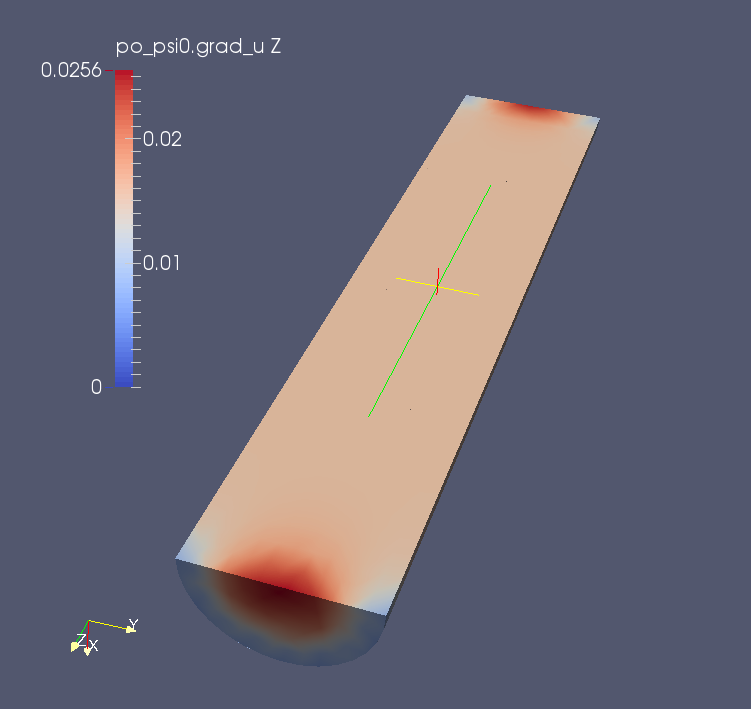
\includegraphics[scale=0.3]{az}}\ 
  \subfloat{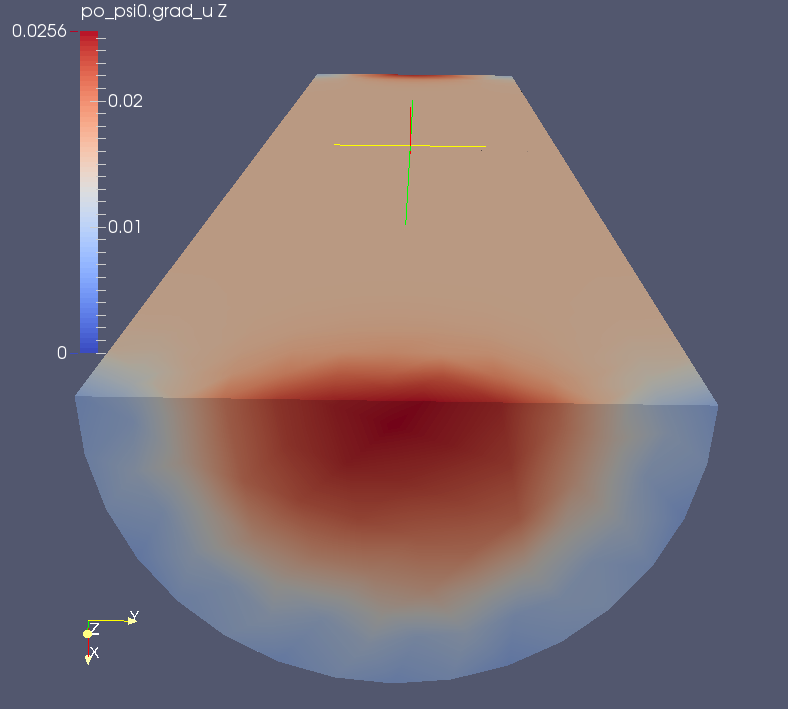
\includegraphics[scale=0.3]{az1}}
}
\caption{$\mathbf{a}=\grad\psi^0\in H(div)$}
\label{az}
\end{figure}

\section{Modes propres}

\section{Problème spectral}


%%% Local Variables:
%%% TeX-master: "../report.tex"
%%% End:
